% Drawing 147/07-2 -- folder 147, batch 07, archive page 140 (PDF page 141).
% Transcription: la même boucle épaissie en une bande hachurée transversalement, les deux branches de la bande se croisant au point double.
% Kind: thickened loop: hatched band crossing itself. Method 2 (schematic redraw from the facsimile). Status: ok.
% Notes: The same loop thickened into a band hatched transversally, the two branches of the band crossing at the double point (dot). The hatching is drawn at regular steps, not stroke for stroke.
% Coordinates: 1 unit = 1 mm = 1/100 of the crop width (bbox in page fractions: [0.366, 0.237, 0.564, 0.408]).
% Redrawn by Claude (claude-opus-5-5), issue #73, 2026-11-07; not checked by a human; not compiled (no TeX in the session).
% Rights: reproduces part of the work -- behind RENDER_TRANSCRIPTS, never published by itself.
\documentclass[tikz,border=3pt]{standalone}
\usepackage{amsmath,amssymb}
\usetikzlibrary{patterns,arrows.meta}
\tikzset{pencil/.style={black!45}, struck/.style={black!35}, mark/.style={circle,draw,inner sep=1.3pt}, pt/.style={circle,fill,inner sep=0.9pt}, opt/.style={circle,draw,fill=white,inner sep=1.1pt}}
\begin{document}
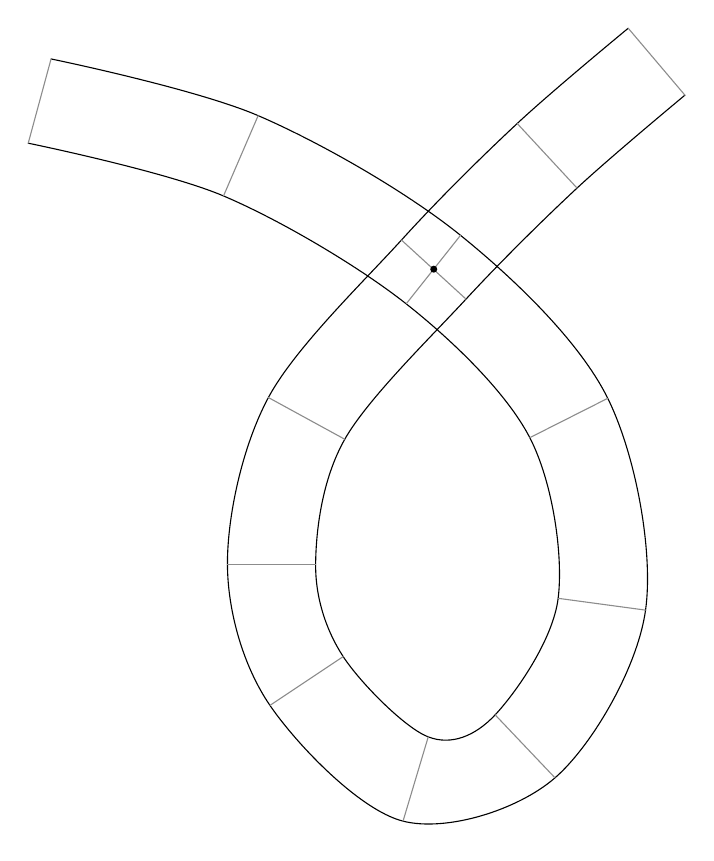
\begin{tikzpicture}[x=1mm,y=1mm,line cap=round,line join=round,font=\scriptsize]
\draw plot[smooth, tension=0.55] coordinates {(9.1,-37.3) (33.9,-44) (57.1,-57.7) (72.8,-74.7) (76.4,-95.1) (68.4,-109.9) (59.9,-112.7) (49.1,-102.5) (45.6,-90.8) (49.3,-74.9) (64.7,-57.1) (78.8,-43) (92.5,-31.2)};
\draw plot[smooth, tension=0.55] coordinates {(12,-26.6) (38.3,-33.8) (64,-49) (82.7,-69.7) (87.5,-96.6) (76,-117.9) (56.7,-123.4) (39.8,-108.7) (34.4,-90.8) (39.6,-69.6) (56.5,-49.6) (71.2,-34.8) (85.3,-22.7)};
\draw[pencil] (9.1,-37.3) -- (12,-26.6);
\draw[pencil] (33.9,-44) -- (38.3,-33.8);
\draw[pencil] (57.1,-57.7) -- (64,-49);
\draw[pencil] (72.8,-74.7) -- (82.7,-69.7);
\draw[pencil] (76.4,-95.1) -- (87.5,-96.6);
\draw[pencil] (68.4,-109.9) -- (76,-117.9);
\draw[pencil] (59.9,-112.7) -- (56.7,-123.4);
\draw[pencil] (49.1,-102.5) -- (39.8,-108.7);
\draw[pencil] (45.6,-90.8) -- (34.4,-90.8);
\draw[pencil] (49.3,-74.9) -- (39.6,-69.6);
\draw[pencil] (64.7,-57.1) -- (56.5,-49.6);
\draw[pencil] (78.8,-43) -- (71.2,-34.8);
\draw[pencil] (92.5,-31.2) -- (85.3,-22.7);
\node[pt] at (60.6,-53.3) {};
\end{tikzpicture}
\end{document}
